\newpage
\appendix
\chapter[Trials and Draws To Decision]{The Trials and Draws to Decision in the Box Task}
%\section{Box task trials, something}
\label{appendix_a}

As we have data from 76 participants that have done the box task, we are presenting the order of the boxes in the nine trials they have done. We also include histograms of how many boxes the participants opened before they either chose the majority colour or the test terminated. This is called draws to decision. 

\begin{figure}
    \centering
    \scalebox{0.8}{\begin{tikzpicture}[node distance = 1.2cm]
    \node (1) [red_trial]{}; 
    \node (2)[red_trial, right of=1]{};
    \node (3)[red_trial, right of=2]{};
    \node (4)[blue_trial, right of=3]{};
    \node (5)[red_trial, right of=4]{};
    \node (6)[red_trial, right of=5]{};
    \node (7)[red_trial, right of=6]{};
    \node (8)[red_trial, right of=7]{};
    \node (9)[blue_trial, right of=8]{};
    \node (10)[red_trial, right of=9]{};
    \node (11)[blue_trial, right of=10]{};
    \node (2)[red_trial, right of=11]{};
\end{tikzpicture}}\\
    \vspace{0.1cm}
    \scalebox{0.8}{\begin{tikzpicture}[node distance = 1.2cm]
    \node (1)[blue_trial]{}; 
    \node (2)[red_trial, right of=1]{};
    \node (3)[blue_trial, right of=2]{};
    \node (4)[red_trial, right of=3]{};
    \node (5)[blue_trial, right of=4]{};
    \node (6)[blue_trial, right of=5]{};
    \node (7)[red_trial, right of=6]{};
    \node (8)[blue_trial, right of=7]{};
    \node (9)[red_trial, right of=8]{};
    \node (10)[blue_trial, right of=9]{};
    \node (11)[red_trial, right of=10]{};
    \node (2)[blue_trial, right of=11]{};
\end{tikzpicture}}\\
    \vspace{0.1cm}
    \scalebox{0.8}{\begin{tikzpicture}[node distance = 1.2cm]
    \node (1) [blue_trial]{}; 
    \node (2)[blue_trial, right of=1]{};
    \node (3)[red_trial, right of=2]{};
    \node (4)[blue_trial, right of=3]{};
    \node (5)[red_trial, right of=4]{};
    \node (6)[blue_trial, right of=5]{};
    \node (7)[red_trial, right of=6]{};
    \node (8)[blue_trial, right of=7]{};
    \node (9)[blue_trial, right of=8]{};
    \node (10)[red_trial, right of=9]{};
    \node (11)[blue_trial, right of=10]{};
    \node (12)[blue_trial, right of=11]{};
\end{tikzpicture}}
    \caption[Order of boxes in the unlimited trials]{The order of the boxes in the three unlimited trials. That is, Trial 2, 3 and 4.}
    \label{fig:unlimited_trials_order}
\end{figure}

\begin{figure}
    \centering
    \scalebox{0.8}{\begin{tikzpicture}[node distance = 1.2cm]
    \node (1)[blue_trial]{}; 
    \node (2)[blue_trial, right of=1]{};
    \node (3)[blue_trial, right of=2]{};
    \node (4)[red_trial, right of=3]{};
    \node (5)[blue_trial, right of=4]{};
    \node (6)[blue_trial, right of=5]{};
    \node (7)[blue_trial, right of=6]{};
    \node (8)[blue_trial, right of=7]{};
    \node (9)[red_trial, right of=8]{};
    
    \node (10)[red_trial, below of=1]{}; 
    \node (11)[blue_trial, right of=10]{};
    \node (12)[blue_trial, right of=11]{};
    \node (13)[red_trial, right of=12]{};
    \node (14)[blue_trial, right of=13]{};
    \node (15)[blue_trial, right of=14]{};
    
    \node (16)[red_trial, below of=10]{}; 
    \node (17)[blue_trial, right of=16]{};
    \node (18)[blue_trial, right of=17]{};
    \node (19)[blue_trial, right of=18]{};
    \node (20)[red_trial, right of=19]{};
    \node (21)[blue_trial, right of=20]{};
    \node (22)[red_trial, right of=21]{};
    \node (23)[blue_trial, right of=22]{};
    \node (24)[blue_trial, right of=23]{};
    
    \node (25)[blue_trial,below of=16]{}; 
    \node (26)[red_trial, right of=25]{};
    \node (27)[blue_trial, right of=26]{};
    \node (28)[red_trial, right of=27]{};
    \node (29)[blue_trial, right of=28]{};
    \node (30)[red_trial, right of=29]{};
    \node (31)[blue_trial, right of=30]{};
    \node (32)[red_trial, right of=31]{};
    \node (33)[blue_trial, right of=32]{};
    
    \node (34)[blue_trial,below of = 25]{}; 
    \node (35)[blue_trial, right of=34]{};
    \node (36)[red_trial, right of=35]{};
    \node (37)[blue_trial, right of=36]{};
    \node (38)[red_trial, right of=37]{};
    \node (39)[blue_trial, right of=38]{};
    
    \node (40)[blue_trial,below of=34]{}; 
    \node (41)[blue_trial, right of=40]{};
    \node (42)[blue_trial, right of=41]{};
    \node (43)[red_trial, right of=42]{};
    \node (44)[blue_trial, right of=43]{};
    \node (45)[blue_trial, right of=44]{};
\end{tikzpicture}}
    \caption[Order of the boxes in the limited trials]{The order of the boxes in the six limited trials. That is, Trials 5, 6, 7, 8 , 9 and 10. We see that Trials 5, 7 and 8 terminate after nine boxes are opened, whereas the other trials terminate after six boxes are opened.}
    \label{fig:all_limited_trials_order}
\end{figure}

\begin{comment}
\begin{figure}	
	\begin{subfigure}{1\textwidth}
		\scalebox{0.8}{\begin{tikzpicture}[node distance = 1.2cm]
    \node (1)[blue_trial]{}; 
    \node (2)[blue_trial, right of=1]{};
    \node (3)[blue_trial, right of=2]{};
    \node (4)[red_trial, right of=3]{};
    \node (5)[blue_trial, right of=4]{};
    \node (6)[blue_trial, right of=5]{};
    \node (7)[blue_trial, right of=6]{};
    \node (8)[blue_trial, right of=7]{};
    \node (9)[red_trial, right of=8]{};
\end{tikzpicture}}
	\end{subfigure}
	\\
	\vfill
	%\vspace{0.5cm}
	\begin{subfigure}{1\textwidth}
		\scalebox{0.8}{\begin{tikzpicture}[node distance = 1.2cm]
    \node (1)[red_trial]{}; 
    \node (2)[blue_trial, right of=1]{};
    \node (3)[blue_trial, right of=2]{};
    \node (4)[red_trial, right of=3]{};
    \node (5)[blue_trial, right of=4]{};
    \node (6)[blue_trial, right of=5]{};
\end{tikzpicture}}
	\end{subfigure}
	\\
	\vfill
	%\vspace{0.2cm}
	\begin{subfigure}{1\textwidth}
		\scalebox{0.8}{\begin{tikzpicture}[node distance = 1.2cm]
    \node (1)[red_trial]{}; 
    \node (2)[blue_trial, right of=1]{};
    \node (3)[blue_trial, right of=2]{};
    \node (4)[blue_trial, right of=3]{};
    \node (5)[red_trial, right of=4]{};
    \node (6)[blue_trial, right of=5]{};
    \node (7)[red_trial, right of=6]{};
    \node (8)[blue_trial, right of=7]{};
    \node (9)[blue_trial, right of=8]{};
\end{tikzpicture}}
	\end{subfigure}
	\\	%\vspace{0.2cm}
	\vfill
	\begin{subfigure}{1\textwidth}
		\scalebox{0.8}{\begin{tikzpicture}[node distance = 1.2cm]
    \node (1)[blue_trial]{}; 
    \node (2)[red_trial, right of=1]{};
    \node (3)[blue_trial, right of=2]{};
    \node (4)[red_trial, right of=3]{};
    \node (5)[blue_trial, right of=4]{};
    \node (6)[red_trial, right of=5]{};
    \node (7)[blue_trial, right of=6]{};
    \node (8)[red_trial, right of=7]{};
    \node (9)[blue_trial, right of=8]{};
\end{tikzpicture}}
	\end{subfigure}
	\\%\vspace{0.2cm}
	\vfill
	\begin{subfigure}{1\textwidth}
		\scalebox{0.8}{\begin{tikzpicture}[node distance = 1.2cm]
    \node (1)[blue_trial]{}; 
    \node (2)[blue_trial, right of=1]{};
    \node (3)[red_trial, right of=2]{};
    \node (4)[blue_trial, right of=3]{};
    \node (5)[red_trial, right of=4]{};
    \node (6)[blue_trial, right of=5]{};
\end{tikzpicture}}
	\end{subfigure}
	\\%\vspace{0.2cm}
	\vfill
	\begin{subfigure}{1\textwidth}
		\scalebox{0.8}{\begin{tikzpicture}[node distance = 1.2cm]
    \node (1)[blue_trial]{}; 
    \node (2)[blue_trial, right of=1]{};
    \node (3)[blue_trial, right of=2]{};
    \node (4)[red_trial, right of=3]{};
    \node (5)[blue_trial, right of=4]{};
    \node (6)[blue_trial, right of=5]{};
\end{tikzpicture}}
	\end{subfigure}
	\caption[Order of the boxes in the limited trials]{The order of the boxes in the six limited trials. That is, Trials 5, 6, 7, 8 , 9 and 10. We see that Trials 5, 7 and 8 terminate after nine boxes are opened, whereas the other trials terminate after six boxes are opened.}
	\label{fig:limited_trials_order}
\end{figure}
\end{comment}


\begin{figure}
    \centering
    \begin{subfigure}{0.48\textwidth}
        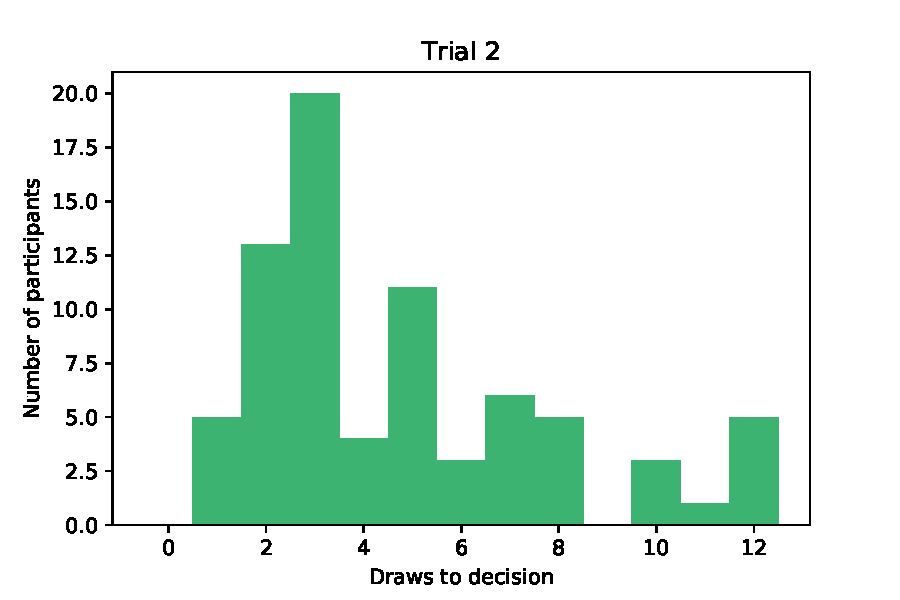
\includegraphics[scale=0.36]{pictures/dtd2_histogram.pdf}
    \end{subfigure}
    \hfill
    \begin{subfigure}{0.48\textwidth}
        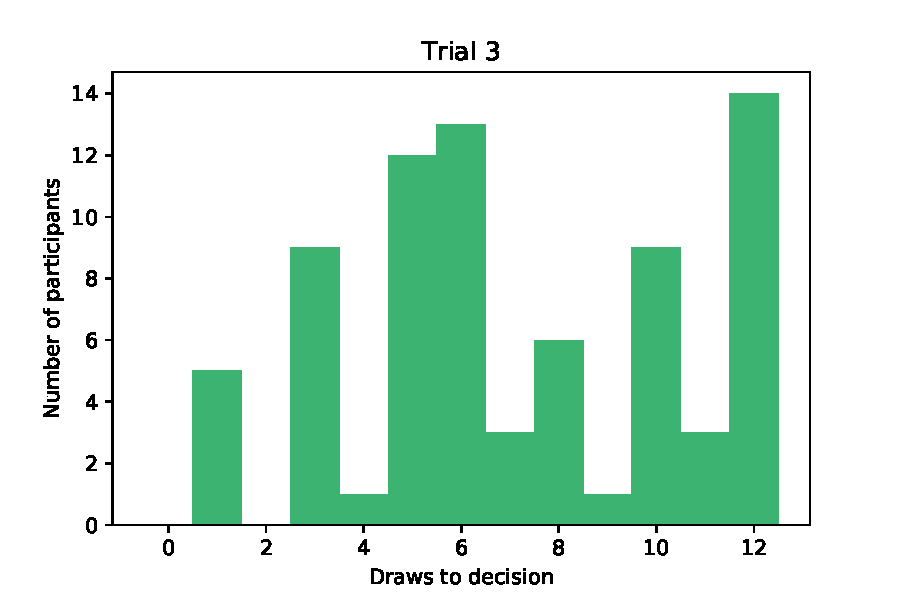
\includegraphics[scale=0.36]{pictures/dtd3_histogram.pdf}
    \end{subfigure}
    \vfill
    \begin{subfigure}{0.48\textwidth}
        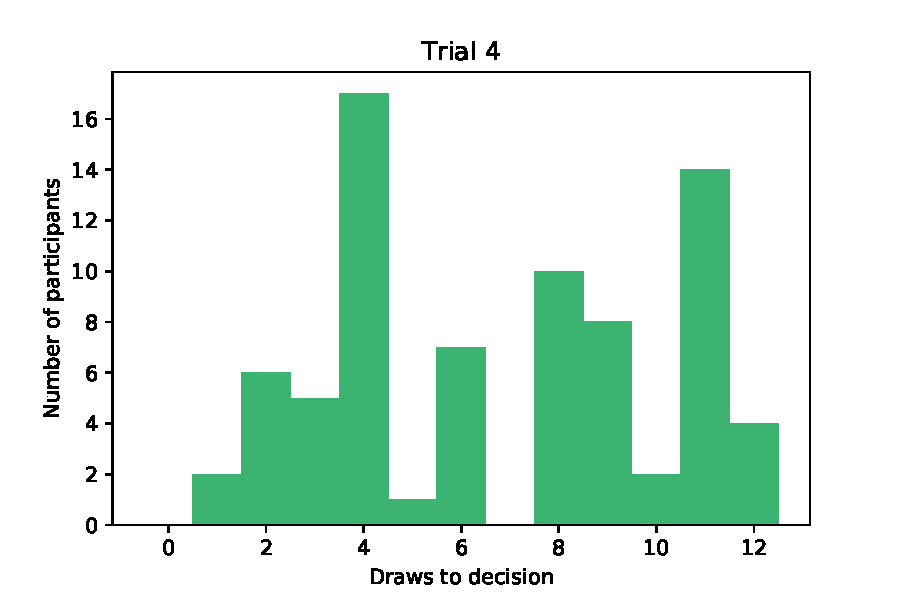
\includegraphics[scale=0.36]{pictures/dtd4_histogram.pdf}
    \end{subfigure}
    \caption[Draws to decision in the unlimited trials]{Histogram of the draws to decisions for all participants in the three unlimited trials.}
    \label{fig:dtd_unlimited_trials}
\end{figure}


\begin{figure}
    \centering
    \begin{subfigure}{0.48\textwidth}
        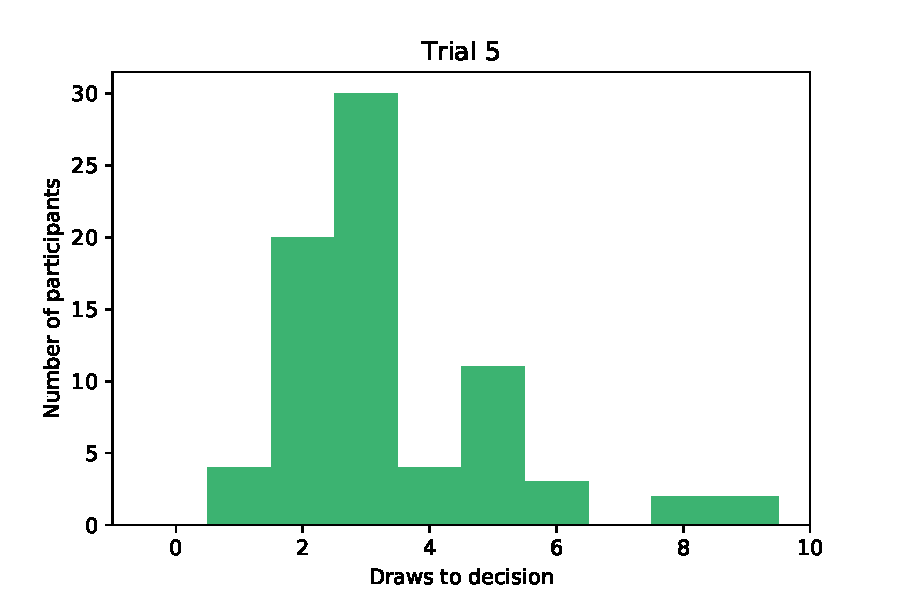
\includegraphics[scale=0.36]{pictures/dtd5_histogram.pdf}
    \end{subfigure}
    \hfill
    \begin{subfigure}{0.48\textwidth}
        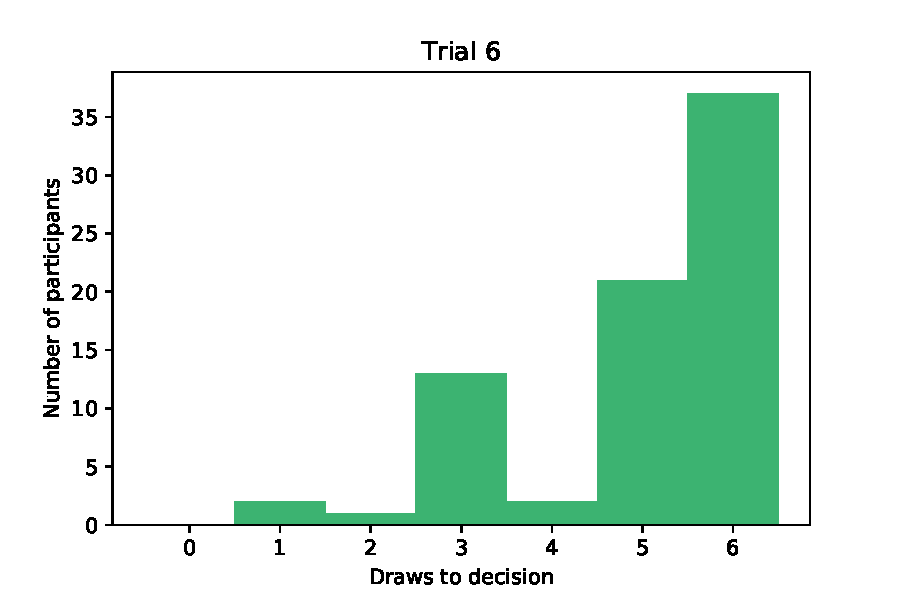
\includegraphics[scale=0.36]{pictures/dtd6_histogram.pdf}
    \end{subfigure}
    \vfill
    \begin{subfigure}{0.48\textwidth}
        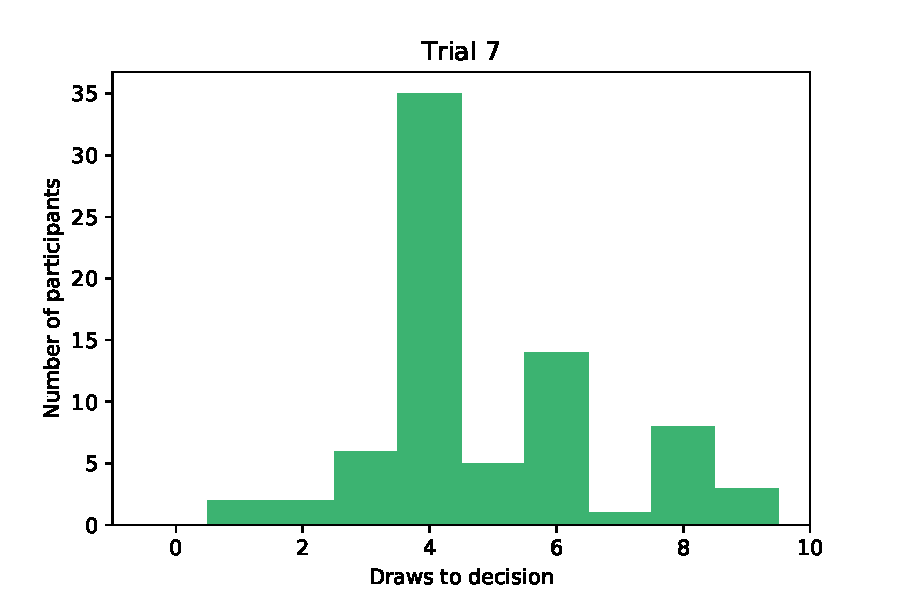
\includegraphics[scale=0.36]{pictures/dtd7_histogram.pdf}
    \end{subfigure}
    \hfill
    \begin{subfigure}{0.48\textwidth}
        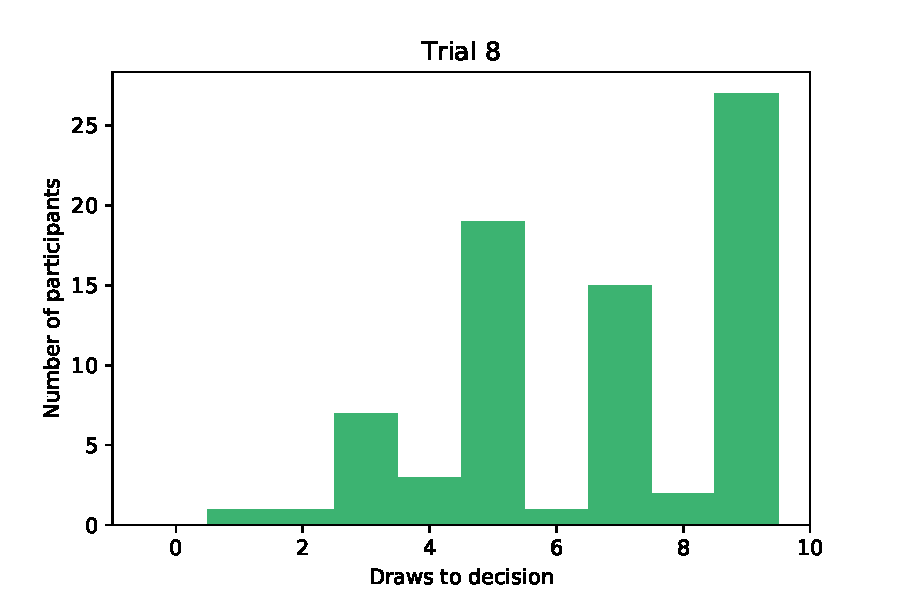
\includegraphics[scale=0.36]{pictures/dtd8_histogram.pdf}
    \end{subfigure}
     \vfill
    \begin{subfigure}{0.48\textwidth}
        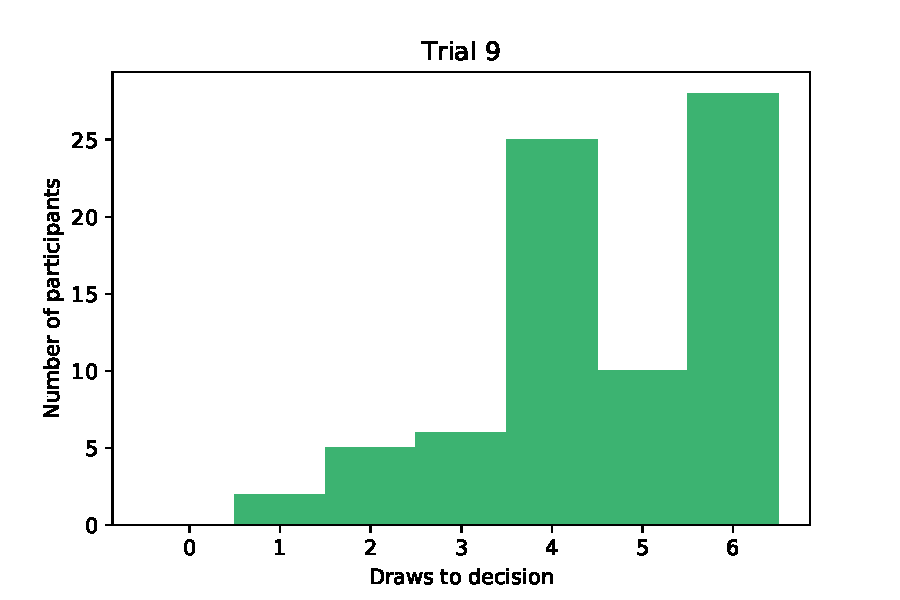
\includegraphics[scale=0.36]{pictures/dtd9_histogram.pdf}
    \end{subfigure}
    \hfill
    \begin{subfigure}{0.48\textwidth}
        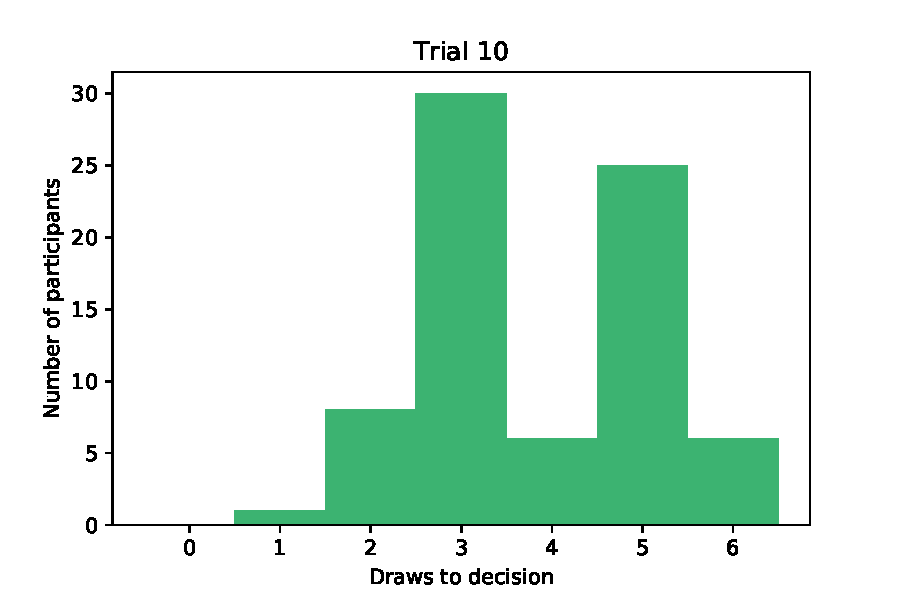
\includegraphics[scale=0.36]{pictures/dtd10_histogram.pdf}
    \end{subfigure}
    \caption[Draws to decision in the limited trials]{The draws to decisions for all participants in the six limited trials. That is, how many boxes they open before they choose what they think is the majority colour, or before the test terminates.}
    \label{fig:dtd_limited_trials}
\end{figure}


\chapter{Confidence Intervals}
\label{appendix_CIs}
\begin{figure}
    \centering
    %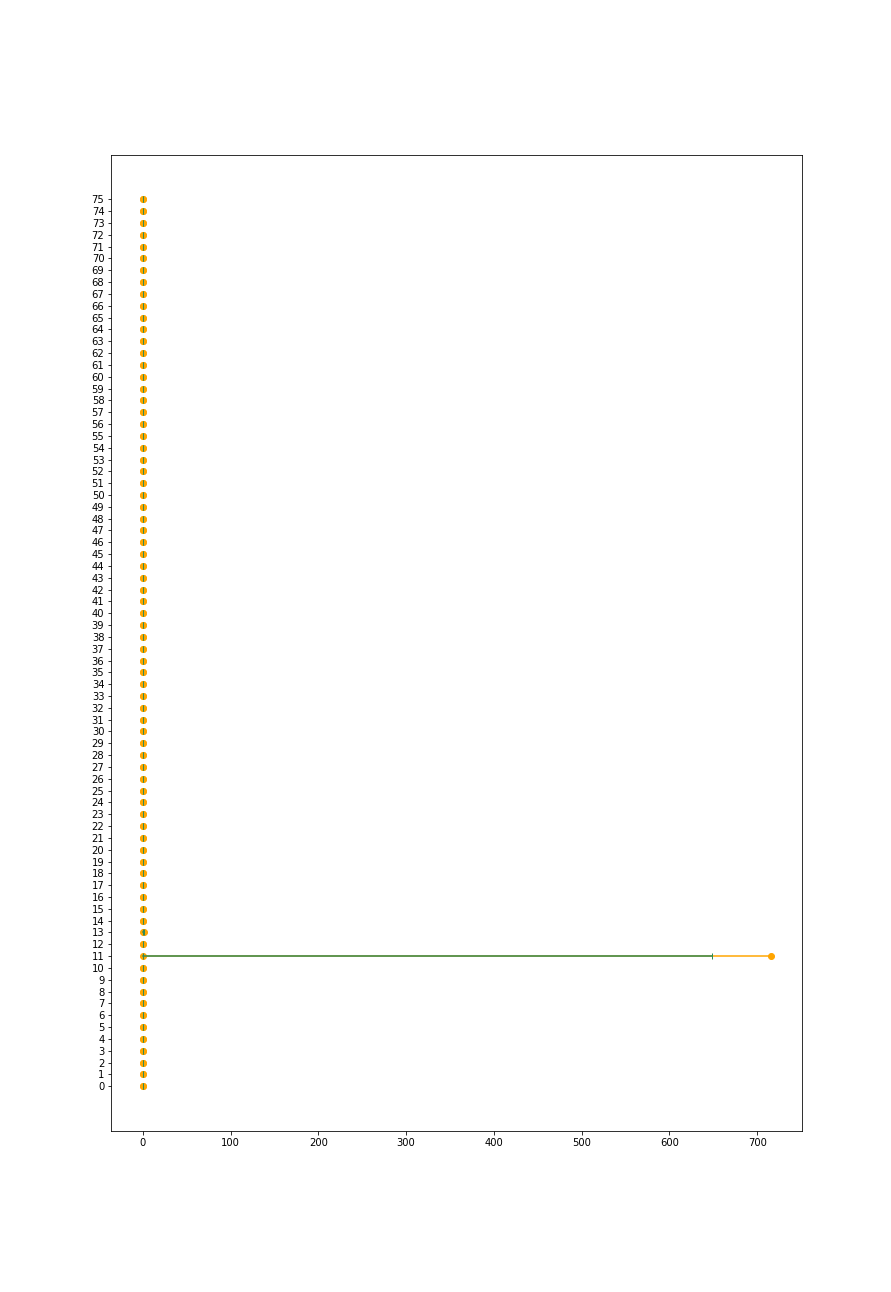
\includegraphics[scale=0.36]{pictures/Sensitivity/ci_lim_alpha.png}
    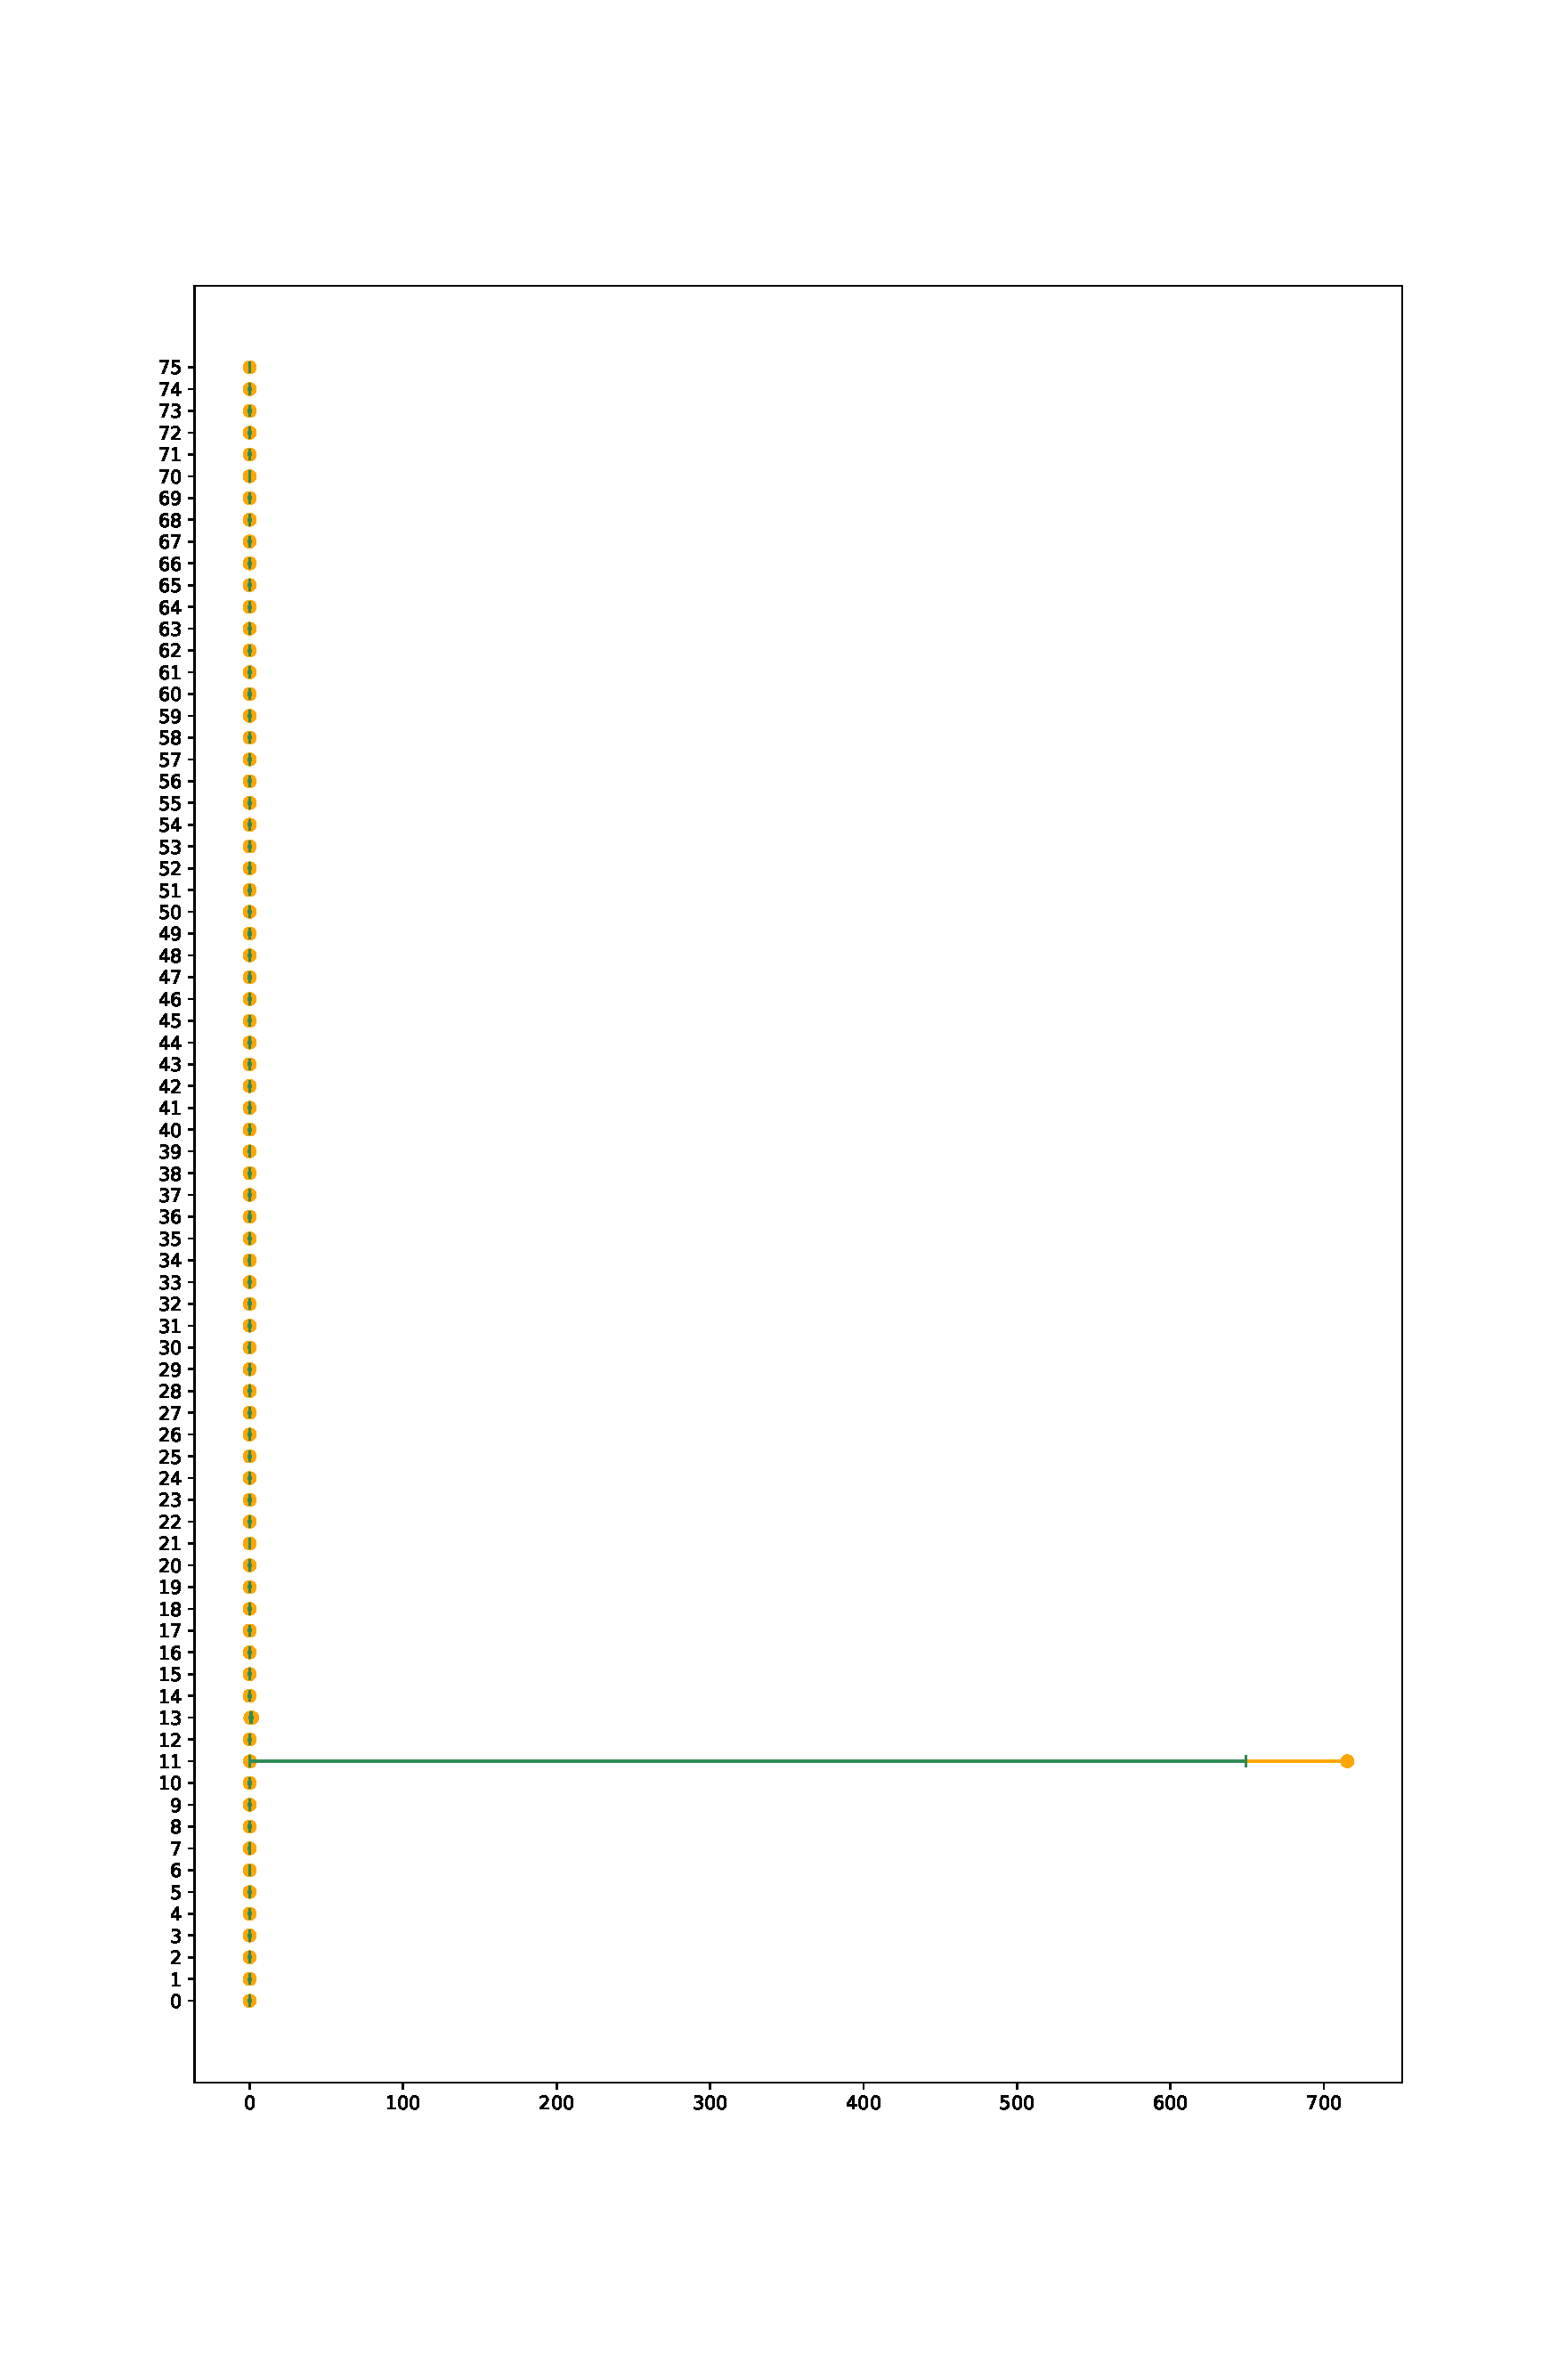
\includegraphics[scale=0.36]{pictures/Sensitivity/ci_lim_alpha_pdf.pdf}
    \caption[CIs for $\alpha$ in the limited case]{Confidence intervals of $\alpha$ in the limited case for all participants with two different priors for $\Theta$. The green lines represent CIs in the situation where we use a uniform prior, that is $\gamma=\kappa=1$ and the orange lines for when we have $\gamma=\kappa=0.5$.}
    \label{fig:sensitivity_cis_lim_alpha}
\end{figure}


\begin{figure}
    \centering
    %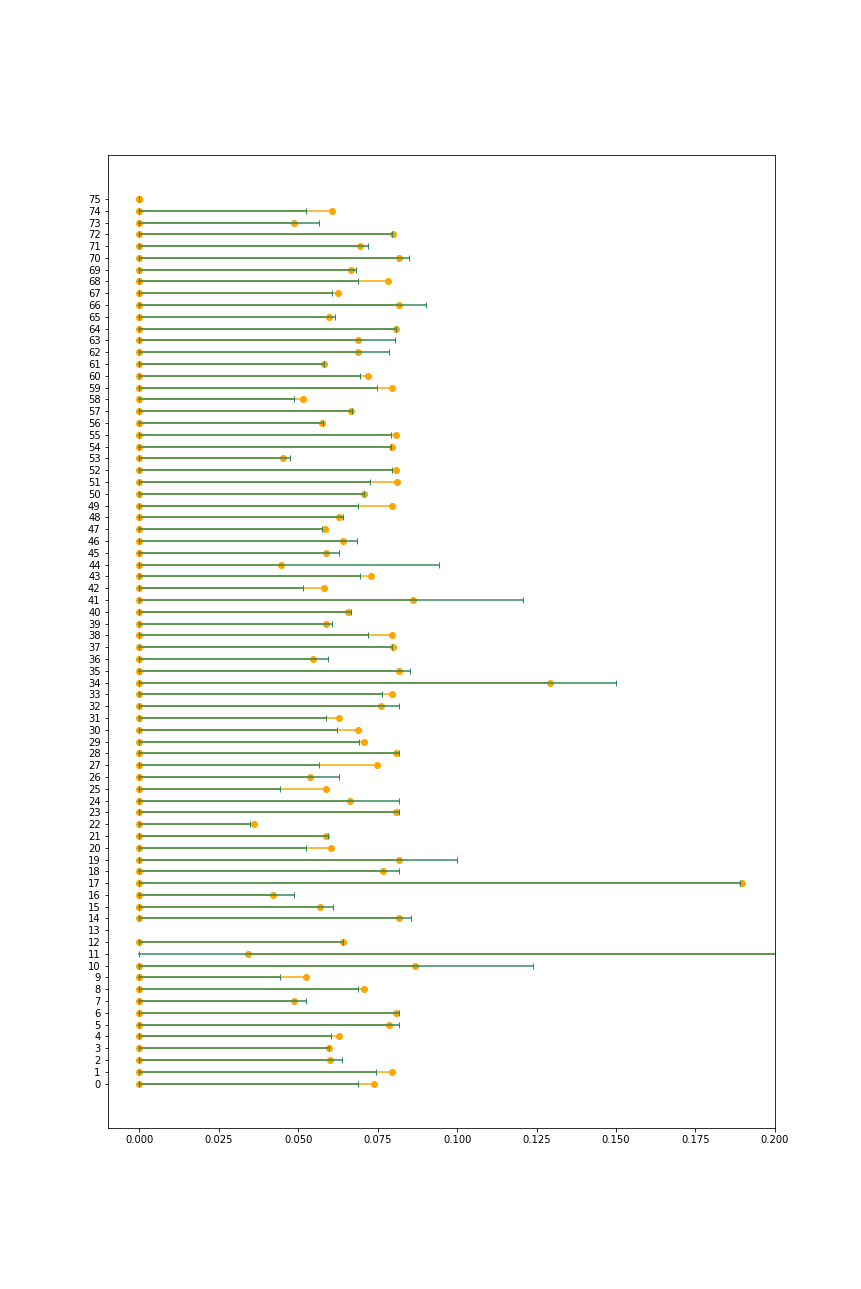
\includegraphics[scale=0.36]{pictures/Sensitivity/ci_lim_alpha_zoom2.png}
    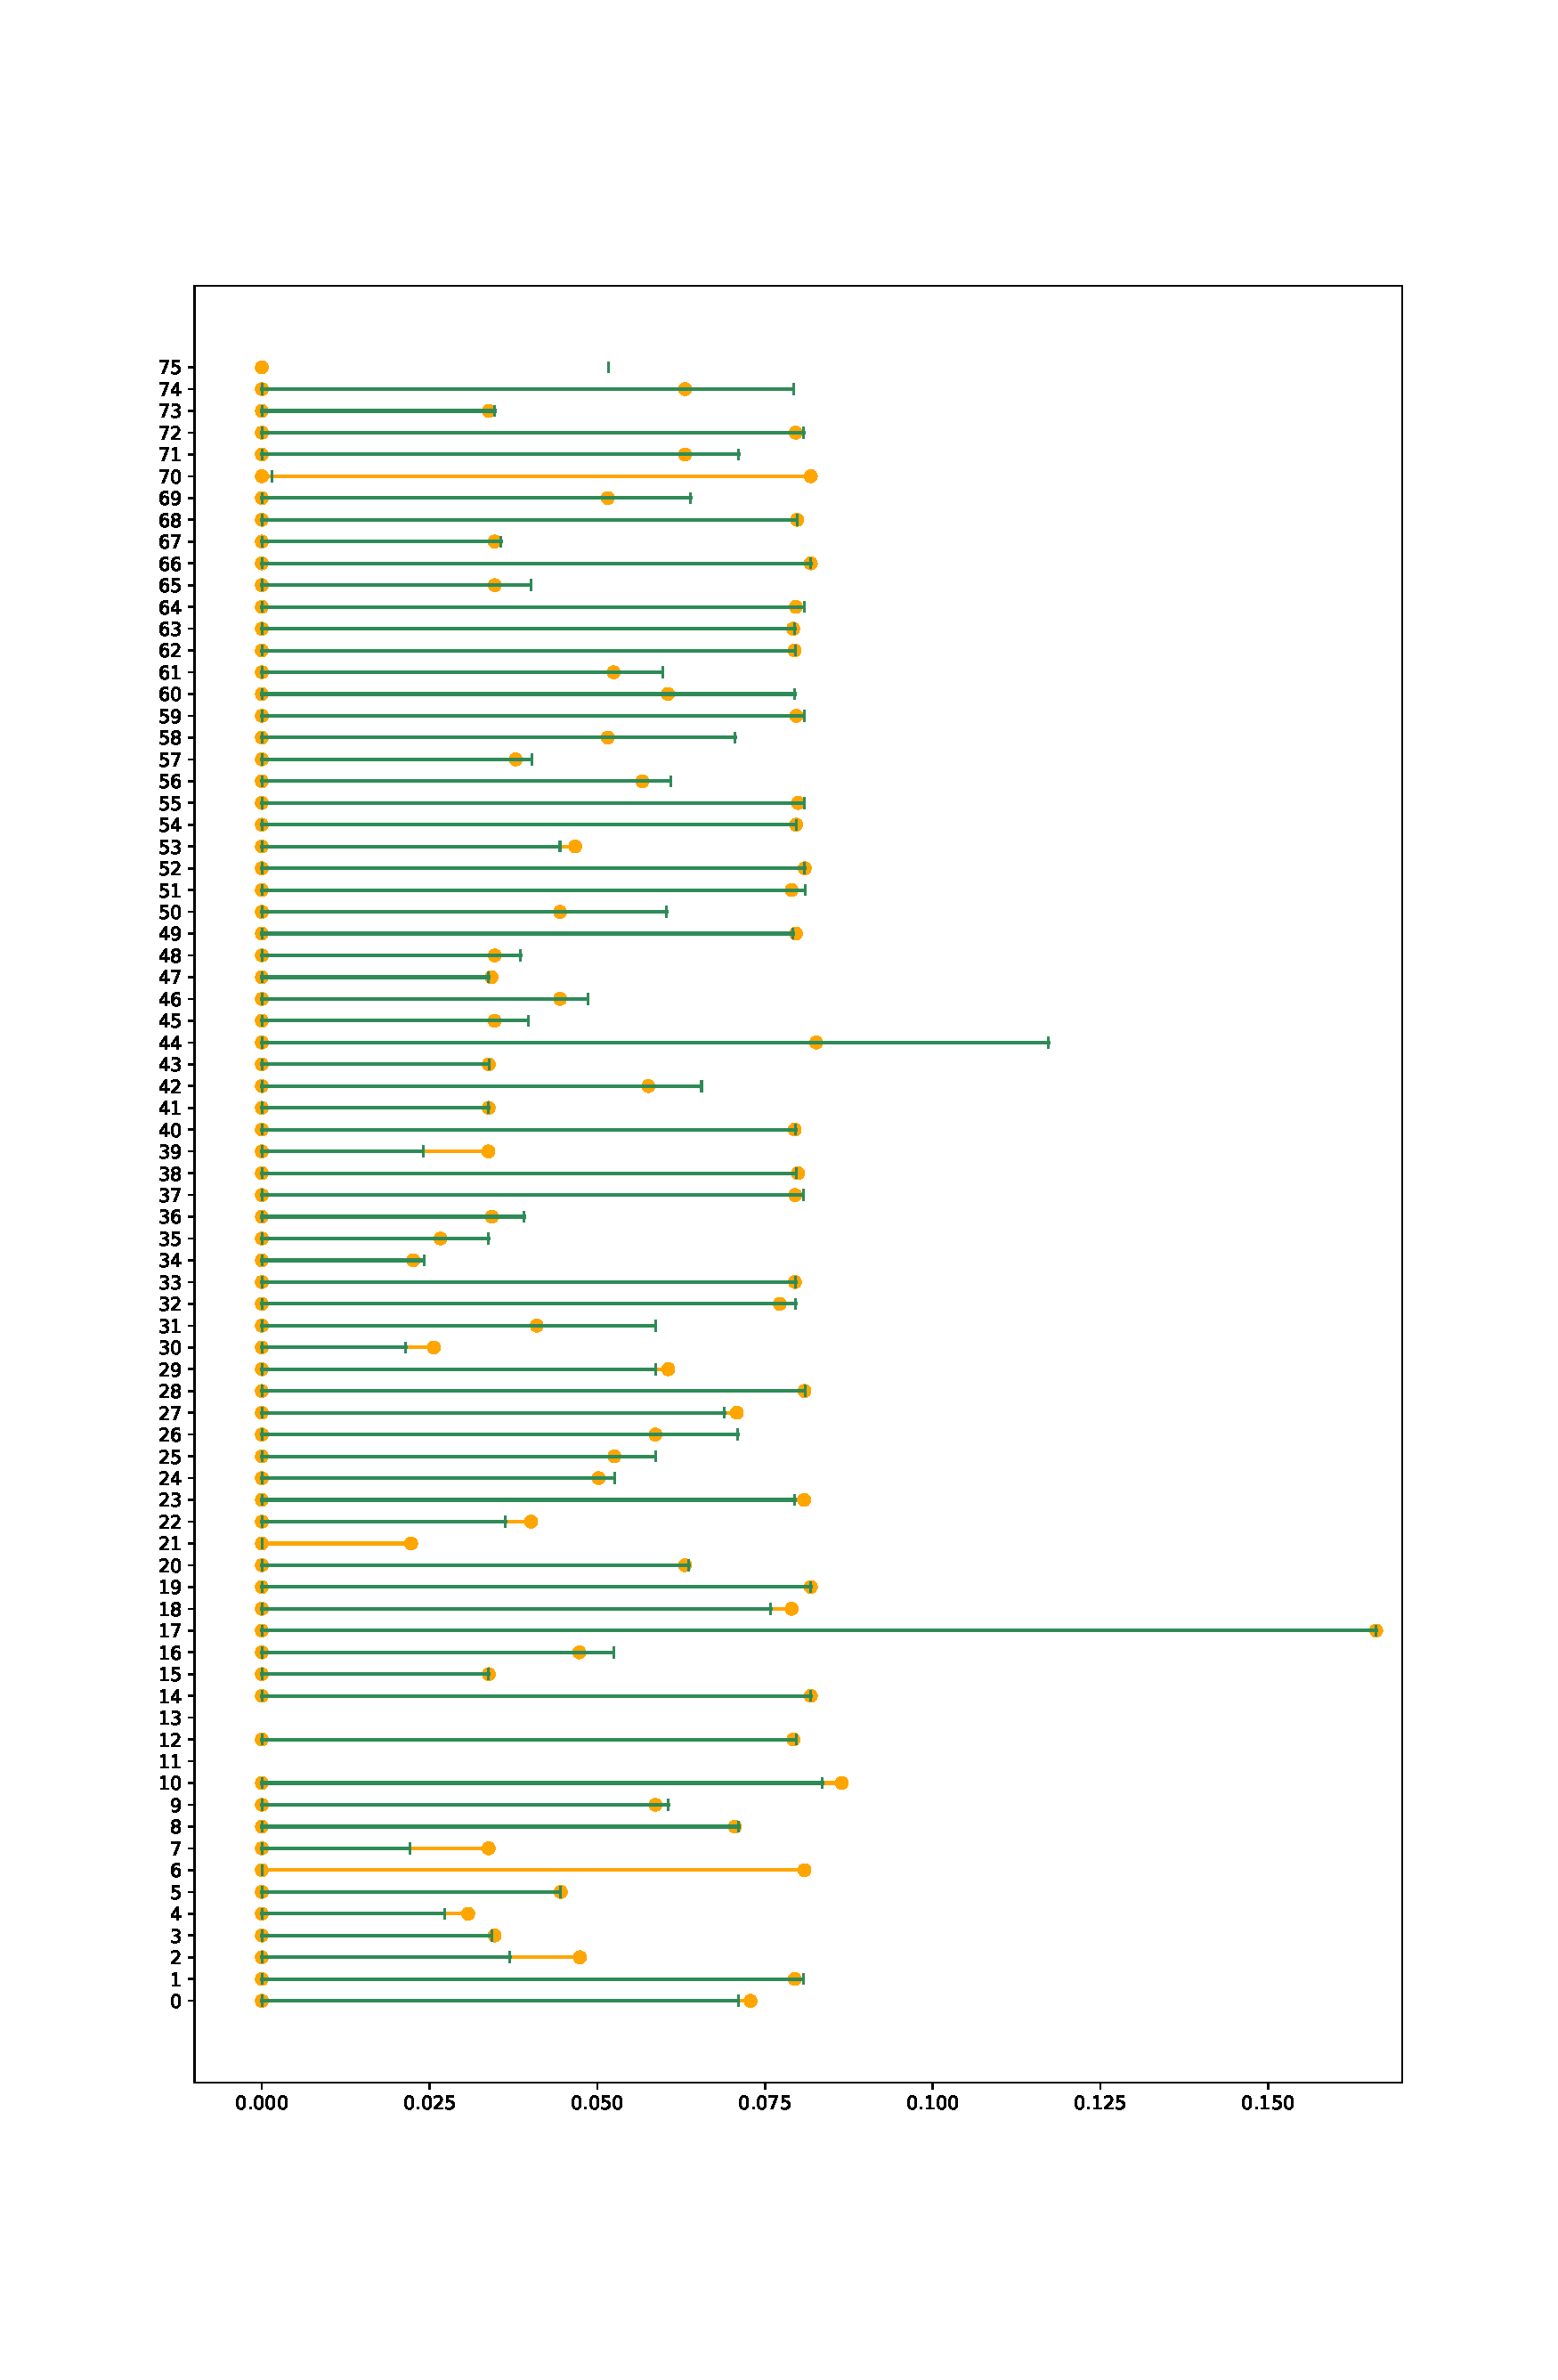
\includegraphics[scale=0.36]{pictures/Sensitivity/ci_lim_alpha_zoom2_pdf.pdf}
    \caption[CIs for $\alpha$ in the limited case, zoomed]{   Confidence intervals of $\alpha$ in the limited case for all participants with two different priors for $\Theta$. Here we have zoomed in more on the plot in Figure \ref{fig:sensitivity_ci_lim_alpha_zoom1}}
    \label{fig:sensitivity_cis_lim_alpha_zoom2}
\end{figure}

\begin{figure}
    \centering
    %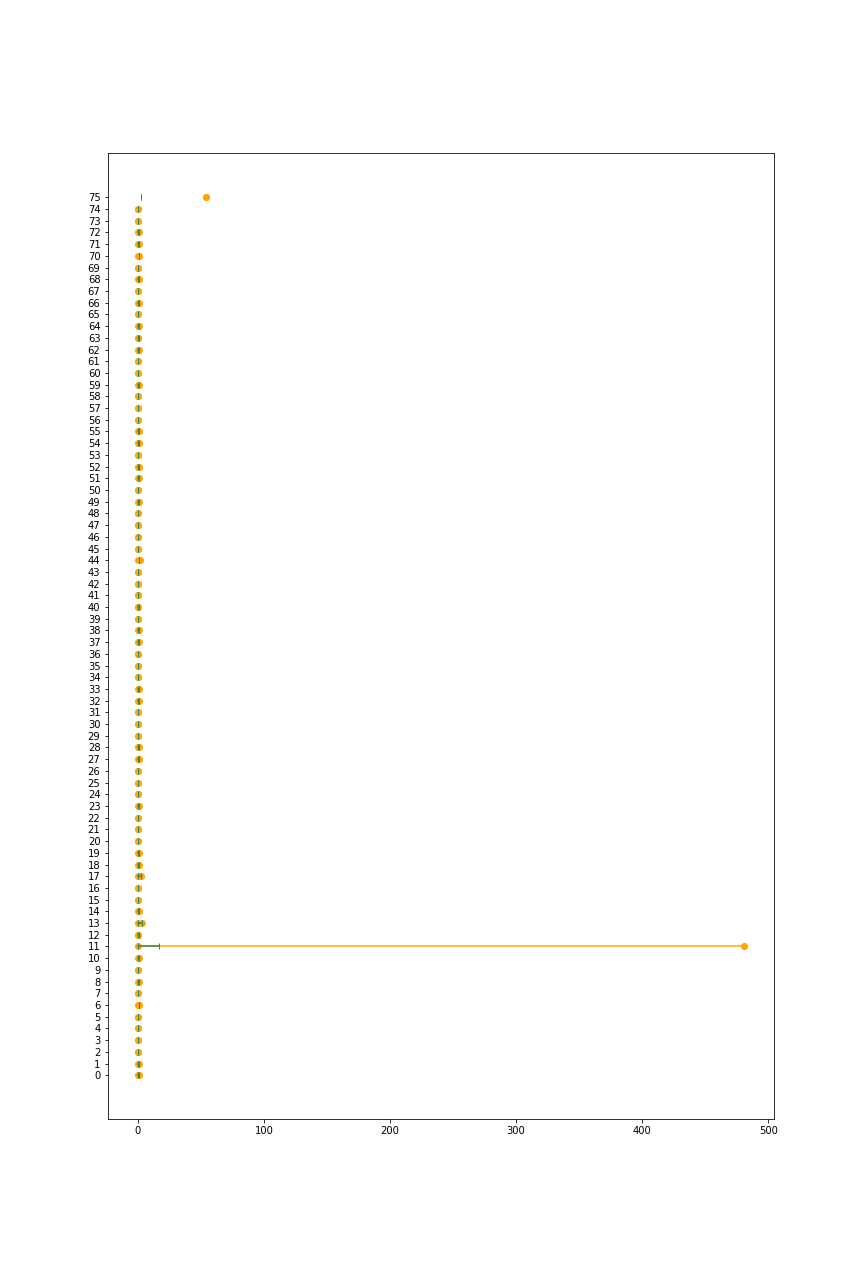
\includegraphics[scale=0.37]{pictures/Sensitivity/ci_lim_beta.png}
    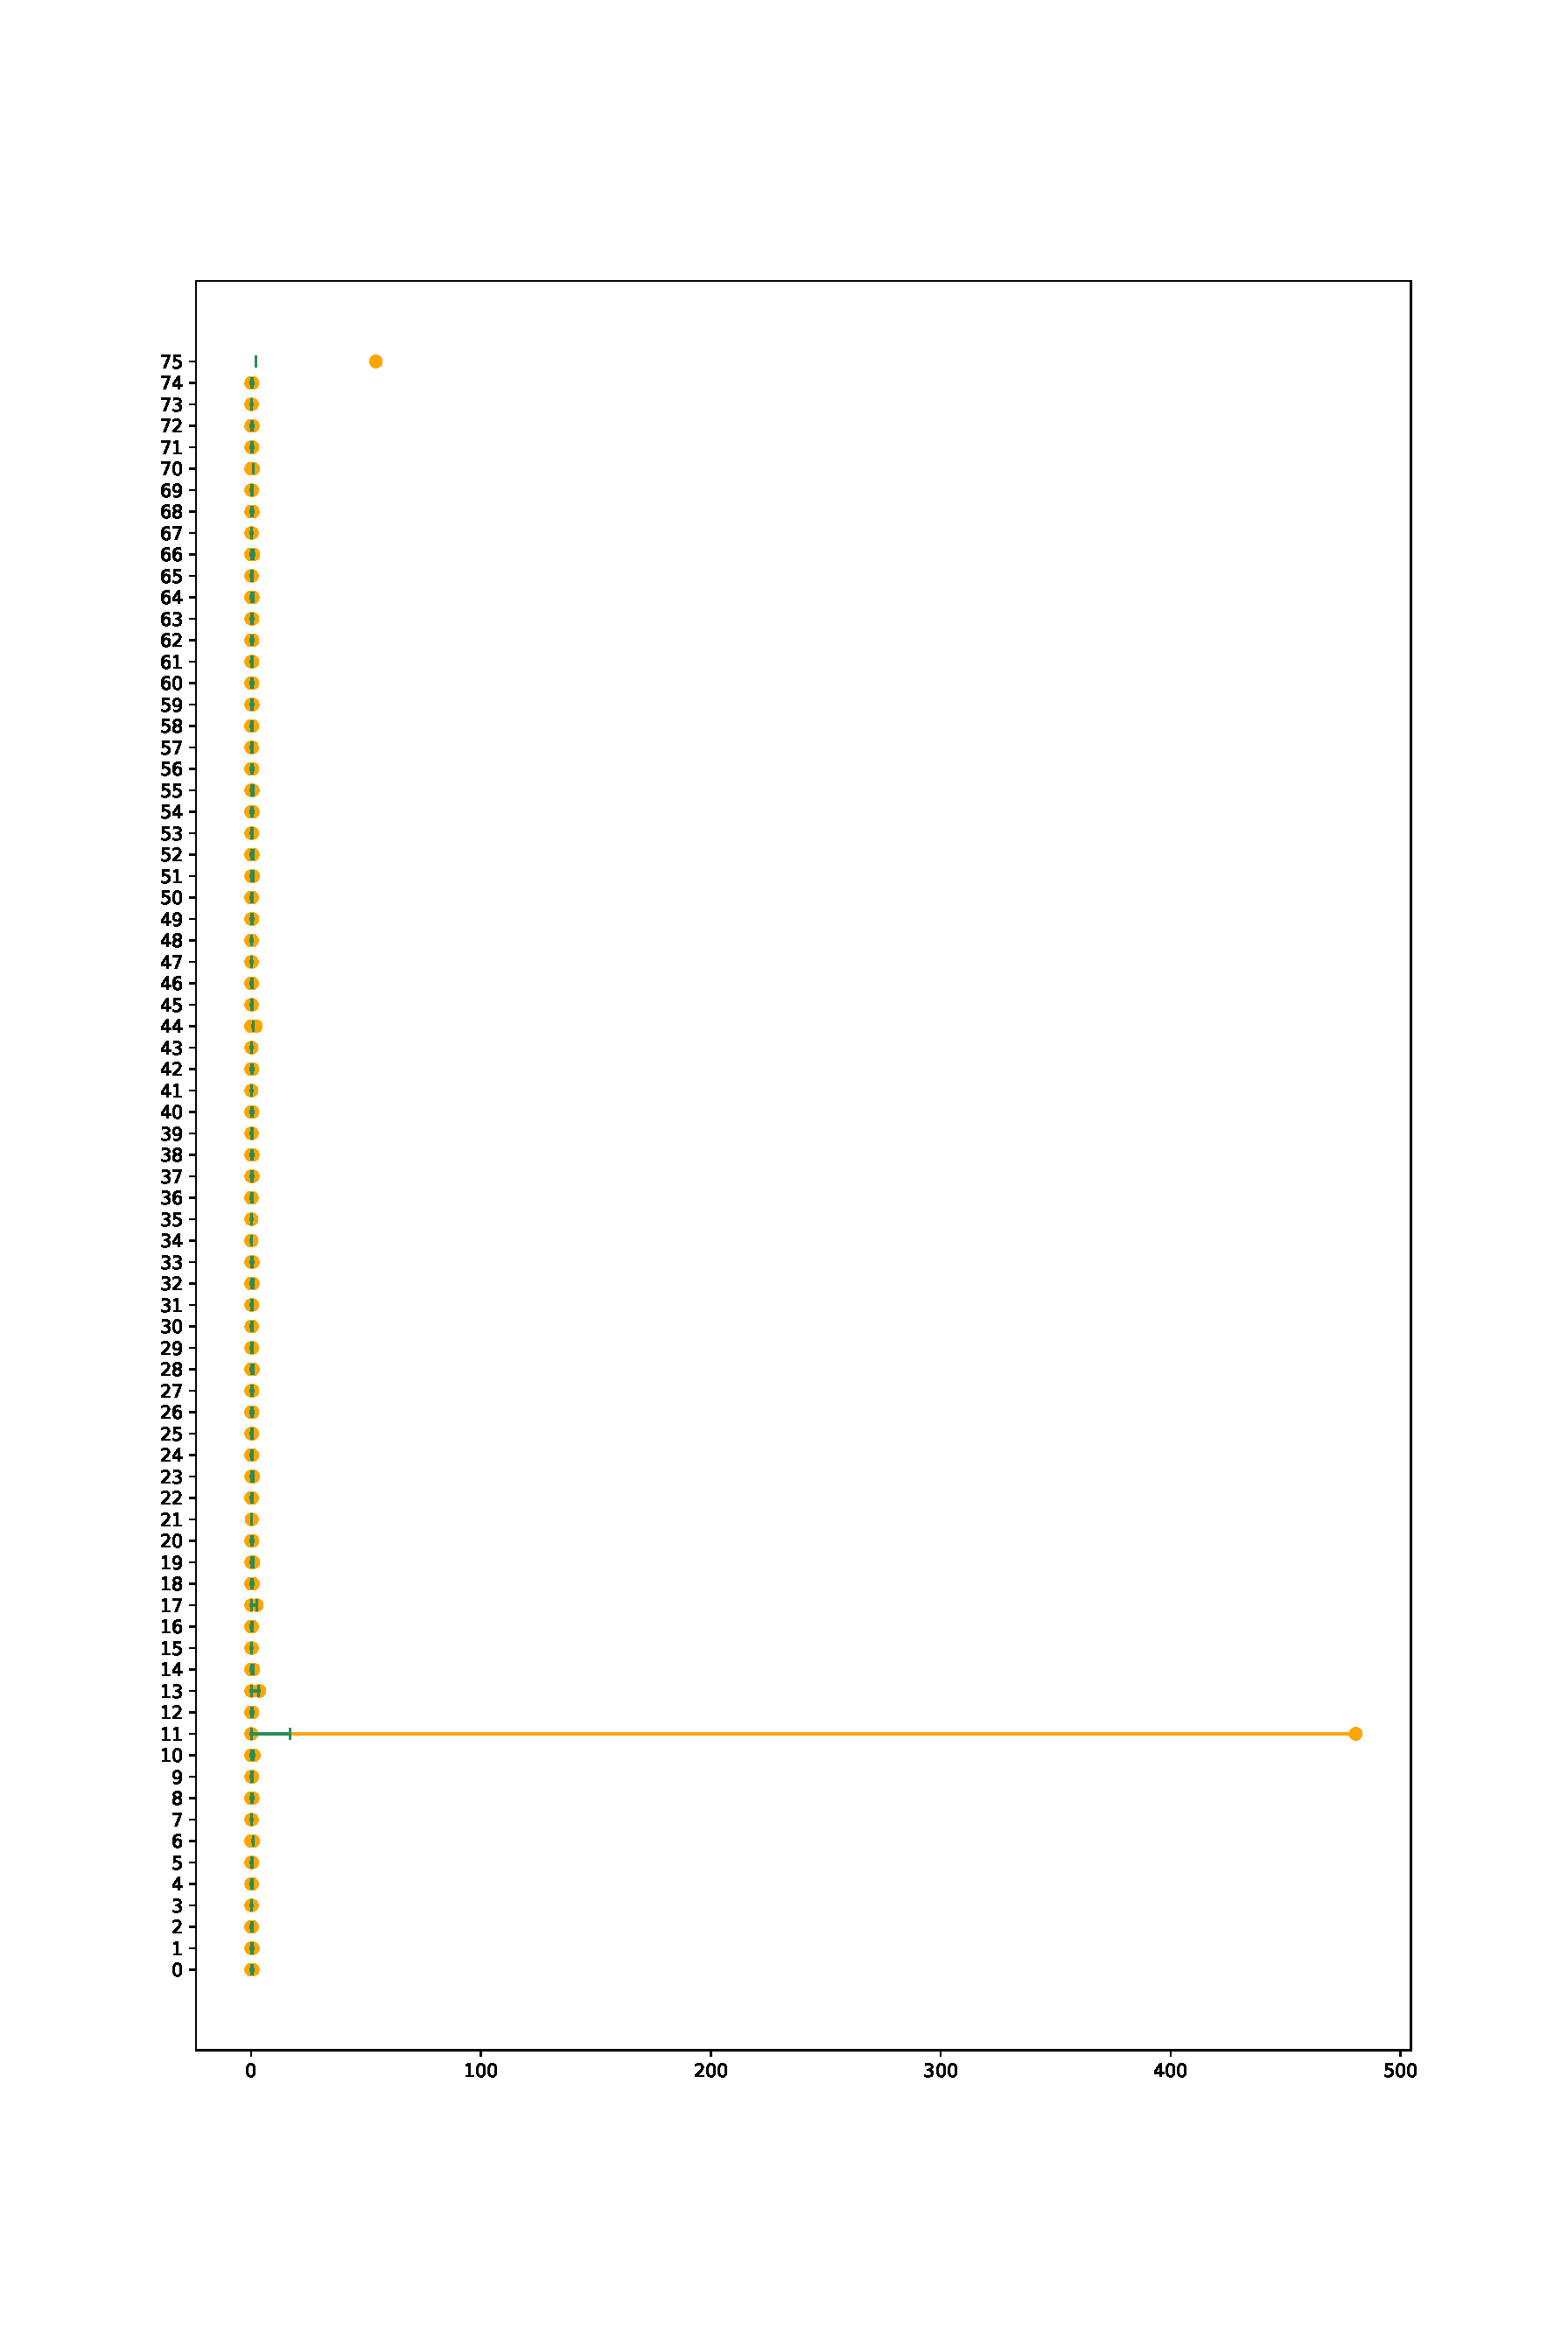
\includegraphics[scale=0.37]{pictures/Sensitivity/ci_lim_beta_pdf.pdf}
    \caption[CIs for $\beta$ in the limited case]{Confidence intervals of $\beta$ in the limited case for all participants with two different priors for $\Theta$. The green lines represent CIs in the situation where we use a uniform prior, that is $\gamma=\kappa=1$ and the orange lines for when we have $\gamma=\kappa=0.5$.}
    \label{fig:sensitivity_ci_lim_beta}
\end{figure}

\begin{figure}
    \centering
    %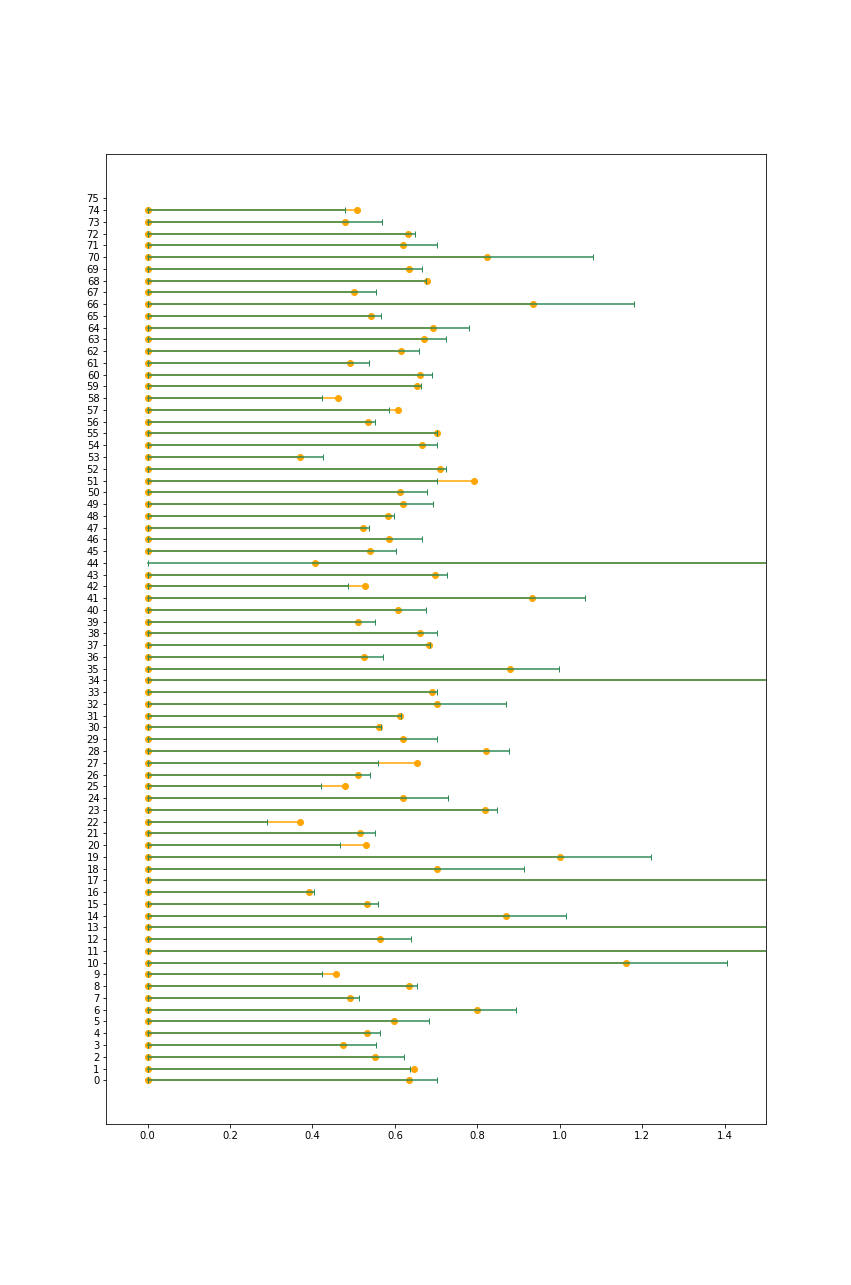
\includegraphics[scale=0.37]{pictures/Sensitivity/ci_lim_beta_zoom2.png}
    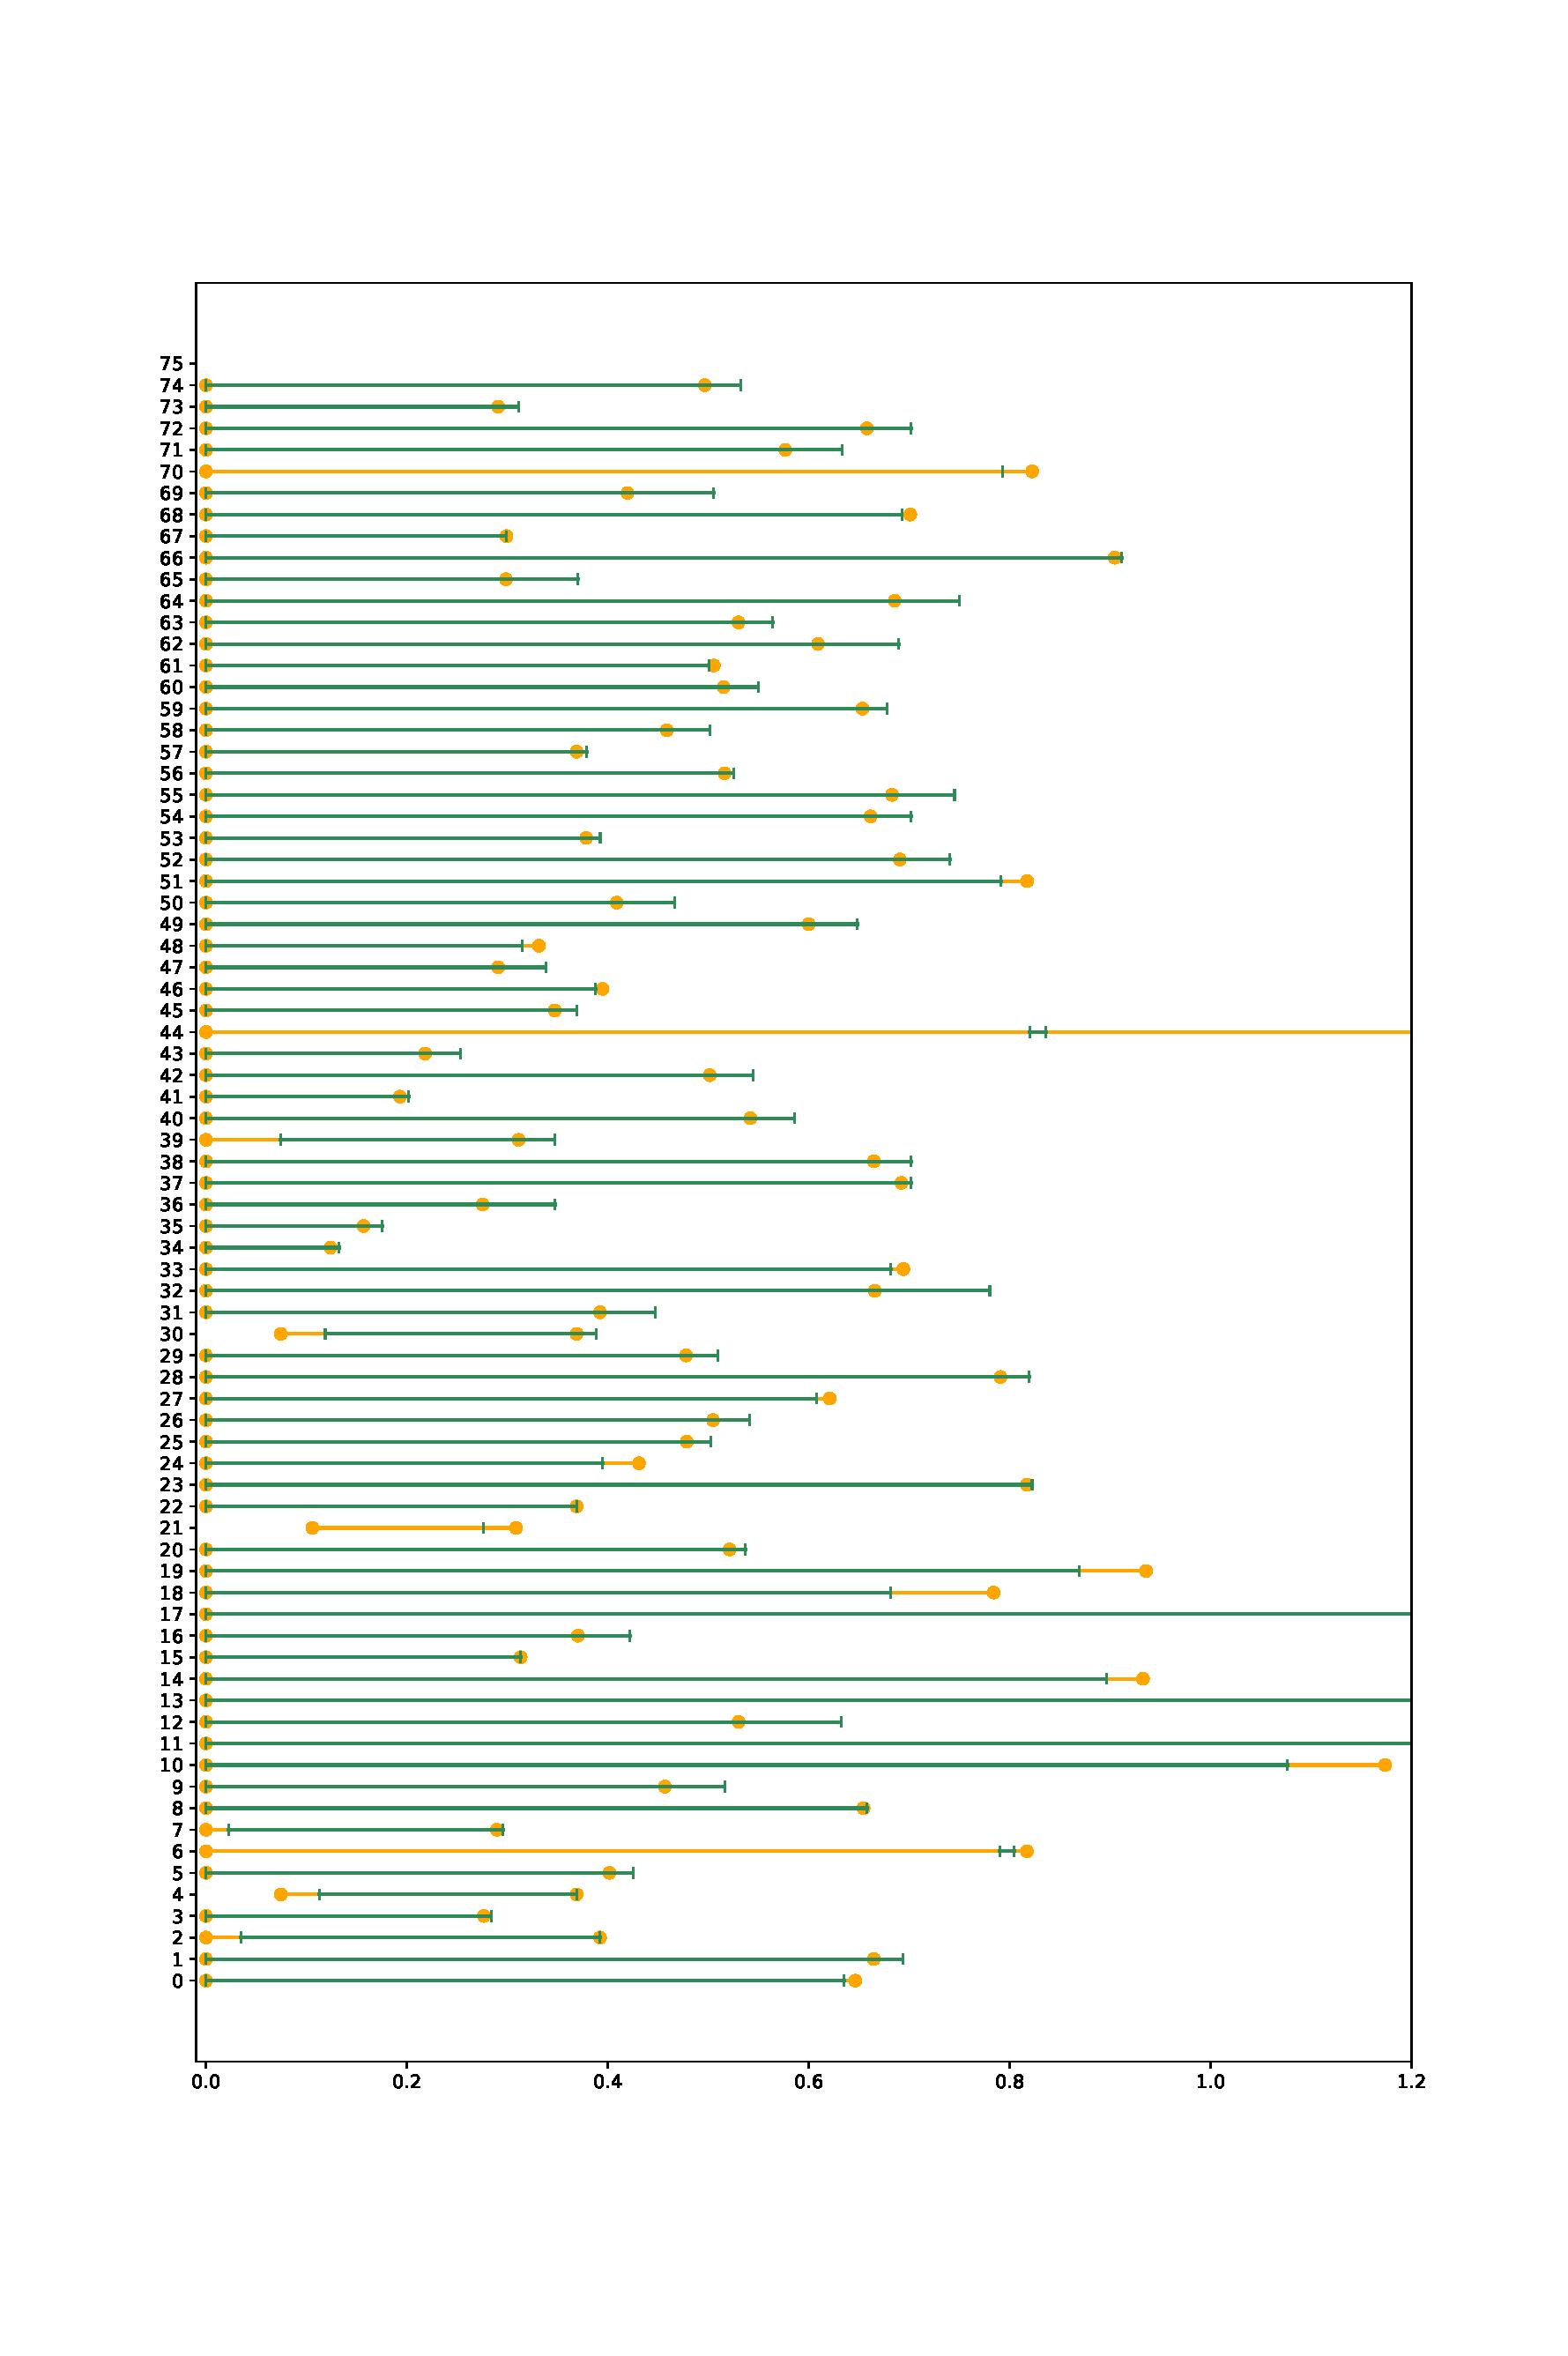
\includegraphics[scale=0.37]{pictures/Sensitivity/ci_lim_beta_zoom2_pdf.pdf}
    \caption[CIs for $\beta$ in the limited case]{Confidence intervals of $\beta$ in the limited case for all participants with two different priors for $\Theta$. Here we have zoomed in on the plot in Figure \ref{fig:sensitivity_ci_lim_beta_zoom}}
    \label{fig:sensitivity_ci_lim_beta_zoom2}
\end{figure}